\cleardoublepage
\clearpage{}

%[Lo que va en el índice]{Lo que va en el documento}
\chapter[Fundamentos]{Fundamentos}
A lo largo de este capítulo se hablará de los \textcolor{brown}{sistemas de archivos} que van a ser objeto de estudio y de las investigaciones que hay alrededor de ellos. Se hará una breve descripción sobre qué \textcolor{magenta}{son y cuales serán objeto de estudio en este proyecto.} \\

Se abordarán los conceptos relevantes que atañen a los \textcolor{brown}{sistemas de archivos}, como pueden ser los métodos de asignación de espacio. Intentaremos definir las estructuras de datos habituales en máquinas Linux, cuáles son y para qué se utilizan. 


\section{Información adicional sobre sistemas de archivos.}
En el capítulo anterior se definió qué era un \textcolor{magenta}{S.A}. En esta sección vamos a profundizar en las partes que lo componen y hablaremos sobre los métodos de reserva de espacio utilizados más comunes.\\

Linux contempla a todos los \textcolor{brown}{sistemas de archivos} como un conjunto de objetos, dichos objetos se dividen principalmente en cuatro categorías. La primera de ellas, el superbloque (\textit{superblock}) se encarga de describir la estructura y \textcolor{magenta}{almacena el estado de este}. \\


 La segunda categoría de objeto encontramos al inodo, el cual contiene metadatos que utiliza el S.A para especificar qué tipo de operaciones se pueden hacer sobre esos objetos. El tercer tipo es la entrada de directorio (\textit{dentry}). Por último, tenemos el objeto archivo, que representa un archivo abierto el cual esta asociado a un proceso \cite{jones_2007}. A continuación se profundizará en cada uno de los objetos citados.\\


\subsection{Superbloque}
El superbloque es una estructura que representa el \textcolor{brown}{sistema de archivos} como un conjunto. Almacena toda la información necesaria para manejarlo, es decir, contiene el nombre, tamaño y estado, un puntero al dispositivo y a los metadatos del \textcolor{magenta}{S.A}.

\subsection{Inodo}
Un inodo es la estructura de datos que describe y almacena los atributos de un archivo, incluyendo su localización física en el disco. Los inodos son creados en el momento de crear el \textcolor{brown}{sistema de archivos}. Contienen información sobre  el tipo de fichero, sus permisos, el id del propietario y la fecha de la última modificación. En resumen, un inodo almacena toda la información del archivo excepto el nombre, el cual se almacena en una estructura del directorio (\textit{dentry}).

\subsection{Métodos de reserva de bloques}
El problema principal del almacenamiento masivo es decidir como reservar espacio del disco para que sea aprovechado, y el acceso a los ficheros sea rápido. Existen principalmente tres métodos de reserva. Cada uno de estos métodos tiene ventajas y desventajas \cite{silberchatz}.


\subsubsection{Contiguous Allocation}
El método de acceso secuencial requiere que el archivo ocupe un conjunto de bloques contiguos en el disco. La ubicación del archivo está definida por la dirección del primer bloque en el disco y el tamaño del archivo. Debido a que todos los registros se colocan uno al lado del otro, acceder a los archivos secuencialmente es muy rápido. Además, el acceso aleatorio también es rápido, porque solo necesita obtener el bloque de inicio y el tamaño del archivo almacenado en la entrada del directorio para encontrarlo. \cite{silberchatz}.\\ 

\newpage
La dificultad de este sistema de reserva de espacio reside en el momento de localizar espacio para un archivo nuevo. La solución que se le da a este problema, no es más que recorrer el disco hasta encontrar un espacio suficientemente grande donde almacenar el archivo. Este tipo de reserva con el paso del tiempo generará bastante fragmentación \cite{silberchatz}.

\begin{figure}[H]
    \centering
    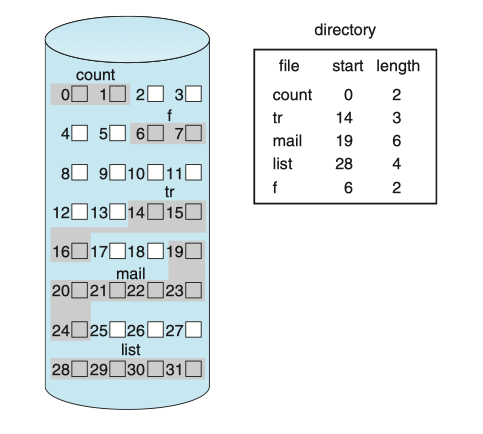
\includegraphics[scale=0.65]{doc/assets/images/Allocation Methods/continuous.png}
    \caption{ \textcolor{magenta}{En la figura se muestra el método de reserva contigua. Se puede ver como los archivos de la tabla están almacenados siguiendo este tipo de reserva }\cite{silberchatz}.}
    \label{fig:my_label}
\end{figure}

%\textcolor{blue}{DE NUEVO COMO DICE ALBERTO EN SU COMENTARIO, LAS FIGURAS SI NO SON TUYAS TIENEN QUE LLEVAR EN EL CAPTION D DONDE SALEN. POR EJEMPLO, SOURCE: URLDELAIMAGEN.COM. ADEMAS, LOS CAPTION DEBEN SER AUTODESCRIPTIVOS, QUE SE ENTIENDA LA IMAGEN MAS O MENOS SIN LEER EL TEXTO, NO VALE CON PONER SOLO EN ESTE CASO EL METODO DE RESERVA.}


\subsubsection{Linked Allocation}
Esta técnica de acceso utiliza listas enlazadas de los bloques que ocupa cada archivo. La entrada de directorio de un archivo contiene punteros al primer y al último bloque de datos del archivo. Cada bloque de datos utiliza 4 bytes de su espacio para almacenar un puntero al siguiente bloque. Este esquema es muy efectivo para acceso secuencial , pero no tiene soporte para acceso directo a un único bloque \cite{silberchatz}.\\

Gracias a la utilización de las listas, se elimina la fragmentación externa y permite que los archivos crezcan de manera sencilla. Una de las desventajas que reside en este tipo de asignación es que si en algún momento se corrompe un puntero quedaría parte del archivo inaccesible \cite{silberchatz}.

\begin{figure}[H]
    \centering
    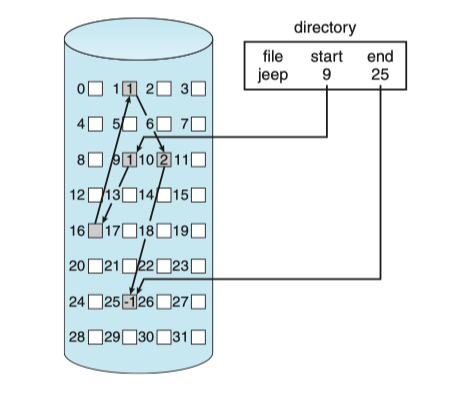
\includegraphics[scale=0.6]{doc/assets/images/Allocation Methods/linked.png}
    \caption{\textcolor{magenta}{ En la figura se muestra un ejemplo de un archivo que cuyo tamaño es de cinco bloques y comienza en el bloque 9, continua en el bloque 16 después en el 1 y en el 10 para finalmente terminar en el bloque 25}  \cite{silberchatz}.}
    \label{fig:my_label}
\end{figure}

\subsubsection{Indexed Allocation}
El acceso indexado resuelve el problema que tenía el acceso enlazado, si se corrompía un puntero. El acceso indexado almacena todos los punteros en una localización: el bloque de índices (\textit{index block}). 
Cada archivo tiene su bloque de índices, el cual es un vector de direcciones de los bloques que componen el archivo \cite{silberchatz}.


\begin{figure}[H]
    \centering
    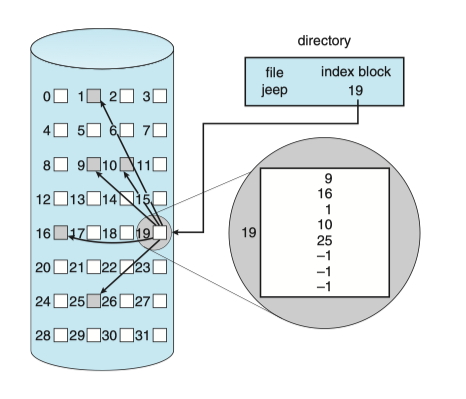
\includegraphics[scale=0.6]{doc/assets/images/Allocation Methods/indexed.png}
    \caption{ \textcolor{magenta}{ Cada archivo tiene su propio bloque de índices, que es un vector de direcciones de bloques de disco. La i-ésima entrada del bloque índice apunta al i-ésimo bloque del archivo. El directorio contiene la dirección del bloque índice \cite{silberchatz}}}
\end{figure}


\section{Introducción a BTRFS}
BTRFS acrónimo de b-tree FS, es un \textcolor{brown}{sistema de archivos} \textit{Copy on Write}. ¿Qué significa esto? Si varios procesos tiene un archivo abierto y uno de ellos lo modifica, dicho cambio cambio de forma transparente, se modificará para que todos los procesos tengan una copia válida del archivo. Utiliza b-trees en su implementación, es decir usa árboles balanceados de búsqueda. Esto hace que BTRFS pueda acceder de manera eficiente a grandes bloques de datos sin importar cuanto crezca el árbol.

\subsection{Características reseñables}
\begin{itemize}
    \item Asignación dinámica de inodos.
    \item Soporte para \textit{snapshots}, subvolúmenes y compresión.
    \item Copia de seguridad incremental.
    \item Defragmentación online.
    \item Tamaño máximo de archivo 16 EiB.
    \item Optimización para discos de estado sólido.
\end{itemize}

\subsection{Diseño de BTRFS}
BTRFS utiliza b-trees para almacenar objetos de distintos tipos. Un b-tree es una estructura de datos, la cual permite que sus nodos tengan más de dos hijos. Al estar implementado bajo un árbol balanceado de búsqueda las operaciones de búsqueda, borrado e inserción se realizan en
\begin{math}
\mathrm{\upvarsigma}(log(n))
\end{math}
\cite{henson}.
\\

Dentro del árbol en las ramas, los nodos almacenan claves y block headers. Las claves  indican dónde buscar el elemento y los block headers señalan dónde se encuentra el próximo nodo en el disco.
Las hojas del árbol almacenan los elementos, que son combinaciones de claves y datos.
\\

BTRFS utiliza un conjunto de código para la manipulación de los metadatos en el \textcolor{brown}{sistema de archivos}. Por motivos de rendimiento u organizativos existen varios b-trees \cite{btrees} que son:
\begin{itemize}
    \item \textbf{\textit{Tree of Tree roots}:} este árbol se usa para indexar  y encontrar la mayoría de raíces de otros árboles dentro del \textcolor{brown}{S.A}. Enlaza nombres a subvolúmenes y \textit{snapshots}, y almacena la ubicación de la raíz del \textit{extent allocation tree}. 
    \item \textbf{\textit{Chunk Tree}:} Es el encargado de realizar el mapeo de direcciones de bloques lógicos a direcciones de bloques físicos. Almacena información sobre todos los dispositivos en el \textcolor{brown}{S.A}. Con el tiempo el árbol se dividirá para dar cabida a almacenamientos más grandes.
    \item \textbf{\textit{Device Allocation Tree}:} Es el árbol encargado de registrar qué partes de un dispositivo físico han sido asignados en chunks. Es un árbol relativamente pequeño, se actualiza solamente cuando un nuevo chunk es asignado. 
    \item \textbf{\textit{Extent Allocation Tree}:} Almacena el rango de bytes que están en uso, el contador de referencias de cada extensión.
    \item \textbf{\textit{FS Tree}:} Almacena archivos y directorios y todos los metadatos que se pueden esperar de estos. Hay un nodo raíz de este árbol por cada subvolumen o snapshot.
    \item \textbf{\textit{Checksum Tree}:} Cada 4000 bloques de datos almacenados en el disco se le asocia un checksum.
\end{itemize}
\newpage
Se puede ver la interconexión de estos b-trees en la siguiente figura: 

\begin{figure}[H]
    \centering
    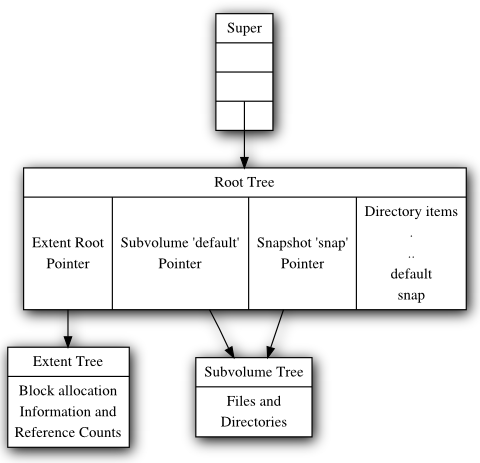
\includegraphics[scale=0.6]{doc/assets/images/btrfs/Design-roots.png}
    \caption{\textcolor{magenta}{ Esquema del la interconexión entre árboles en BTRFS \cite{btrees}}}
    \label{fig:my_label}
\end{figure}


\section{Introducción a Ext4}
Ext4 es el sucesor de Ext3, este \textcolor{brown}{sistema de archivos} es el mas popular entre la distribuciones linux. Ext4 integra cambios sustanciales como puede ser la mejora de las estructuras de datos.

\subsection{Características reseñables}
\begin{itemize}
    \item Defragmentación online.
    \item Tamaño máximo de archivo 16 TiB.
    \item Filesystem check.
    \item Journaling checksumming.
\end{itemize}


\subsection{Diseño de EXT4}
Ext4 está diseñado para ser escalable, en los últimos años los archivos se han ido haciendo mas grandes (sobre todo en temas relacionados con multimedia). Ext4 asegura la escalabilidad gracias a varios aspectos los cuales se detallan a continuación.\\

\subsubsection{Extendiendo los limites del sistema de archivos}
Etx4 se diseñó con vista a la creciente demanda de espacio en los archivos, por ello es capaz de almacenar archivos de hasta 16TB (asumiendo tamaños de bloque de 4KB). También se pensó en eliminar el límite de subdirectorios que existía en Ext3. En Ext3 el limite de subdirectorios era de 32KB mientras que en Ext4 pasó a ser virtualmente ilimitado. Se optimizó la indexación de directorios y en la actualidad Ext4 utiliza un \textit{hashed b-tree}, lo cual hace que el tiempo en búsqueda sea menor que su predecesor. \cite{jones_2009}

\subsubsection{\textit{Extents}}
Un \textit{extent} es una manera simple de representar una contigua secuencia de bloques. Gracias a ello, el tamaño de los metadatos es menor ya que no se almacena la información de donde están los bloques almacenados si no que se almacena una lista de las secuencias de bloques.\\

Para almacenar archivos grandes, un inodo referencia a un nodo índice y este puede hacer referencia a un nodo hoja (que puede referenciar varios extents) tal y como se muestra en la figura.

\begin{figure}[H]
    \centering
    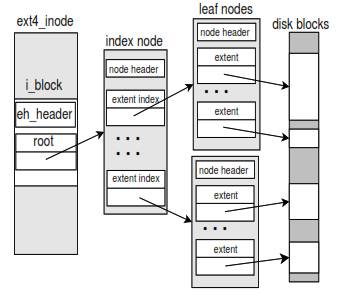
\includegraphics{doc/assets/images/ext4/ext4_map_extent_tree.PNG}
    \caption{\textcolor{magenta}{ Se muestra la disposición del árbol de extensiones. La raíz de este árbol se almacena en la  el inodo y las extensiones se almacenan en los nodos hoja del árbol. \cite{Mathur2007}}}
    \label{fig:Ext4 Extent Tree}
\end{figure}

\subsubsection{\textit{Multiblock Allocation}}
Cuando EXT3 necesita escribir datos nuevos en el disco, hay un \textit{block allocator} que decide cuales van a ser los bloques libres que se van a asignar para escribir los datos. El problema es que este \textit{block allocator} solo es capaz de asignar un bloque, es decir, 4KiB por cada vez que se le llama. Para tener una idea del problema que esto supone, se presenta un ejemplo. Si se requiere escribir 100 MiB, Ext3 necesitará llamar al \textit{block allocator} 25600 veces. Esto no es solo un despropósito en términos de eficiencia, si no que también imposibilita aplicar políticas para optimizar las asignaciones ya que no se sabe cual es el tamaño total del lo que se pretende almacenar. Para solventar los problemas que esto suponía en Ext3, se decidió que en Ext4 se utilizaría un \textit{multiblock allocator}, el cual es capaz de asignar muchos bloques en una sola llamada, en vez de un solo bloque por llamada, disminuyendo así la sobrecarga. Gracias al uso del multiblock allocator mejora el rendimiento si se combina  con \textit{delayed allocation} el cual se definirá  a continuación. \cite{ext4howto} \\


\subsubsection{\textit{Delayed Allocation}}
La asignación retardada o \textit{delayed allocation} es una función que incrementa el rendimiento de los \textcolor{magenta}{S.A}. Esta característica se puede encontrar \textcolor{magenta}{por ejemplo, en} XFS, ZFS, BTRFS o Reiser4. Consiste en retrasar lo máximo posible la asignación de bloques. Por ejemplo, si un proceso ejecuta una operación \textit{write()}, en los \textcolor{magenta}{sistemas de archivos} tradicionales se reservarían los bloques donde esta información va a ser guardada. Dicha aproximación cuenta con algunas desventajas, por ejemplo, si un proceso se encuentra ejecutando un bucle que escribe en un archivo, se estaría asignando espacio continuamente. La asignación retardada por otro lado, no reserva los bloques inmediatamente, si no que mientras que el archivo esta en caché retrasa la reserva hasta que realmente se va a escribir en el disco. 
La reserva retardada o \textit{delayed allocation}, se complementa muy bien con dos funcionalidades previamente mencionadas los \textit{extents} y el \textit{multiblock allocation} \cite{ext4howto}.




\subsection{Fiabilidad}
Ext4 para incrementar su fiabilidad realiza dos tareas principalmente, \textit{journaling} y \textit{checksumming}.\\

\textit{Journaling} es el mecanismo que permite al sistema de ficheros recomponerse en caso de caída en una situación crucial. Para ello, \textcolor{magenta}{se} va escribiendo en un log todas las operaciones que se hacen para que, en caso fatal, no desemboque en una corrupción del \textcolor{brown}{sistema de archivos}. Aun así es posible \textcolor{magenta}{que esto ocurra} y por ello Ext4 implementa un \textit{checksumming} del \textit{journal}, para detectar dicha situación.\\

Otra funcionalidad que implementa este \textcolor{brown}{sistema de archivos} es lo que se conoce como "defragmentación online". Aunque Ext4 esta diseñado para minimizar la fragmentación con el paso del tiempo es prácticamente imposible evitarla, por esta razón es necesaria una herramienta de defragmentación y su funcionamiento se basa en copiar archivos en inodos nuevos que referencia un espacio mas continuo que el anterior.


\section{Introducción a XFS}
XFS es un \textcolor{brown}{sistema de archivos} desarrollado por \textit{Silicon Graphics} en 1993 \textcolor{magenta}{cuyo código} fue liberado en mayo del 2000. \cite{xfs}

\subsection{Características principales}
\begin{itemize}
    \item Tamaño máximo de archivo 8EiB.
    \item Journaling para operaciones con metadatos.
    \item E/S Directa para alto rendimiento y E/S no cacheada para dispositivos DMA.
    \item Snapshots.
    \item Defragmentación online
    \item \textit{Delayed allocation} para minimizar la fragmentación.
    \item Basado en extents donde los archivos pueden tener extents de longitud variable.
\end{itemize}

XFS utiliza tecnología de \textit{journaling} de base de datos para incrementar la fiabilidad y la rapidez en caso de recuperación. XFS es capaz de recuperarse tras un bloqueo del sistema en unos pocos segundos, sin necesidad de usar un comprobador como podría ser \textit{fsck}. El tiempo que tarda XFS en recuperarse es completamente independiente del tamaño.\\

En XFS los inodos se crean \textcolor{magenta}{de forma dinámica conforme el sistema} los va necesitando. En el proceso de creación \textcolor{magenta}{de XFS}, se puede especificar el tamaño de los inodos.\\

XFS permite elegir el tamaño de bloque \textcolor{magenta}{ a la hora de ser creado}. En la documentación de XFS nos recomiendan los siguientes tamaños de bloque \cite{xfs}:

\begin{itemize}
    \item El tamaño mínimo de bloque son 512 bytes. Tamaños de bloque pequeños suponen una sobrecarga en la asignación, lo que conlleva que disminuya el rendimiento. Este tamaño \textit{Sillicon Graphics} lo recomienda para sistemas cuyo tamaño sea inferior a 100 \textit{megabytes} con bastantes archivos pequeños.
    
    \item El tamaño de bloque por defecto en XFS es 4096 bytes es decir 4KB.
    \item El tamaño de bloque máximo es el tamaño de página del kernel en sistemas basados en la arquitectura x86 se trata de 4KB, pero en sistemas basados en ia64 puede ser mayor. \textit{Sillicon Graphics} no recomienda que el tamaño de bloque se exceda de 4KB, ya que tamaños de bloque mayores implicarían probablemente un desperdicio de espacio.
\end{itemize}

\section{Workload Model Language}
WML es un lenguaje que se utiliza para definir benchmarks en Filebench el cual permite a sus usuarios codificar una amplia variedad de cargas de trabajo. Los procesos en WML representan procesos UNIX reales, los cuales son creados por Filebench en tiempo de ejecución. \cite{Tarasov2016FilebenchAF}. 


\section{Estado del arte} \label{estado}
Tal y como se mencionó en el capítulo 1, las investigaciones relacionadas con este tema, no suelen ser todo lo correctas que se desearía. En la mayoría de casos se obvian o se dan por supuestas algunas asunciones, que imposibilitan la crítica del trabajo puesto que no disponemos de todo el conjunto de la información. \\

Se han seleccionado algunas de las investigaciones mas citadas relacionadas con el tema a estudiar con el objetivo de señalar sus puntos débiles.  Además, se pretende mejorar ciertos aspectos de dichas investigaciones en este proyecto.\\

La selección de trabajos ha sido la siguiente.
\begin{itemize}
    \item \textit{Performance Analysis of 64-bit ext4, xfs and btrfs filesystems on the Solid-State disk technology} \cite{Kljaji2016PerformanceAO}.
    
    \item \textit{Benchmarking Performance of Erasure Codes for Linux Filesystem EXT4, XFS and BTRFS} \cite{10.1007/978-981-15-6584-7_32}.
    
    \item \textit{Competition of virtualized ext4, xfs and btrfs filesystems under type-2 hypervisor} \cite{competitionvirtualized}.
    
    \item \textit{Benchmarking Performance of EXT4, XFS and BTRFS as Guest File Systems Under Linux Environment} \cite{serbios}.
    
    \item \textit{Comparative Performance Analysis of Magnetic Hard Disk and Solid-State Drives Using 64-bit btrfs Filesystem} \cite{Stojkov2016ComparativePA}.
    
    \item \textit{Ext4, XFS, BtrFS and ZFS Linux File Systems on RADOS Block Devices (RBD)} \cite{7881982}.
    
    \item \textit{Modern filesystem performance in local multi-disk storage space configuration} \cite{Smolinski2014ModernFP}.
    
\end{itemize}

A continuación se analizará en detalle cada publicación.

\subsubsection{Análisis: Performance Analysis of 64-bit ext4, xfs and btrfs filesystems on the Solid-State disk technology}

Esta publicación tiene como objetivo analizar el rendimiento de ext4, btrfs y xfs en un SSD (\textit{solid state disk}). El benchmark utilizado en esta publicación es \textit{Bonie++} se han realizado operaciones de lectura y escritura tanto secuencial como aleatoria.\\

A lo largo del documento, se ha detectado algunas situaciones que se tratarán de evitar en este trabajo. Por un lado en el documento no se especifica cómo se montan los sistemas de archivos, ni que configuración tienen, por ejemplo no se especifica el tamaño de bloque. Por otro lado en el apartado hardware, sólo se especifica el tamaño de la memoria RAM en ningún momento se menciona la frecuencia ni la latencia. Para finalizar, el disco utilizado para las pruebas es el mismo en el que se aloja el sistema operativo, con el objetivo de interferir lo mínimo posible en la prueba se debería haber utilizado un SSD para albergar las ejecuciones \cite{Kljaji2016PerformanceAO}.\\

\subsubsection{Benchmarking Performance of Erasure Codes for Linux Filesystem EXT4, XFS and BTRFS}
Con el paso de los años el \textit{erasure code} o código de borrado en castellano, se ha ido extendiendo como mecanismo para asegurar la integridad de los datos. El objetivo de la publicación es comparar distintas implementaciones sobre XFS, BTRFS y EXT4. En el apartado en el que se explica la metodología y el hardware a utilizar, no se detalla el modelo de memoria RAM. Tampoco se menciona ninguna característica del disco y debería ser imprescindible que estos datos aparezcan \cite{10.1007/978-981-15-6584-7_32}.


\subsubsection{Competition of virtualized ext4, xfs and btrfs filesystems under type-2 hypervisor}
Esta investigación se centra en el análisis de EXT4, BTRFS y XFS bajo un hipervisor de virtualización de tipo-2. En la metodología aparece de forma detallada las pruebas que se van a realizar, las características del disco duro empleado y el rango de tamaño de los archivos utilizados en las pruebas. Vuelve a ocurrir que no se detalla ninguna característica sobre la memoria RAM \cite{competitionvirtualized}.

\subsubsection{Benchmarking Performance of EXT4, XFS and BTRFS as Guest File Systems Under Linux Environment}
Se parte del objetivo de analizar el rendimiento de tres sistemas de ficheros. En esta prueba se utiliza  \textit{Filebench} para la ejecución de unos test llamados \textit{file server}, \textit{mail server} y \textit{web server}. No se detalla que realiza cada prueba, ni que operaciones en el sistema de archivos realiza. Esta situación se intentará evitar en este trabajo. Respecto a las especificaciones hardware no se especifica el modelo, ni características de la memoria RAM. Como aspecto positivo destacar que la metodología expresa de manera clara y concisa la manera en que los discos estan configurados para la prueba \cite{serbios}.

 \subsubsection{Comparative Performance Analysis of Magnetic Hard Disk and Solid-State Drives Using 64-bit btrfs Filesystem} 
 Se compara el rendimiento de BTRFS uilizando un SSD frente a un HDD. En la publicación se detalla de forma clara el hardware de los discos, pero tal y como sucede en los trabajos anteriores no se dan detalles sobre las especificaciones de la memoria RAM. Para la ejecución de las pruebas se utiliza \textit{Bonie++}. Este test realiza lecturas y escritura tanto como secuenciales como aleatorias \cite{Stojkov2016ComparativePA}.
    
\subsubsection{Ext4, XFS, BtrFS and ZFS Linux File Systems on RADOS Block Devices (RBD)} 
En este articulo tiene como objetivo realizar un análisis comparativo de estos sistemas de ficheros sobre LVM (\textit{logical volume manager}) utilizando ZFS sobre RADOS Block Device. Este trabajo es interesante por la topología de red que utiliza, ya que los distintos discos se encuentran en máquinas diferentes, es decir, se ejecuta en un sistema distribuido \cite{7881982}. 

\begin{figure}[H]
    \centering
    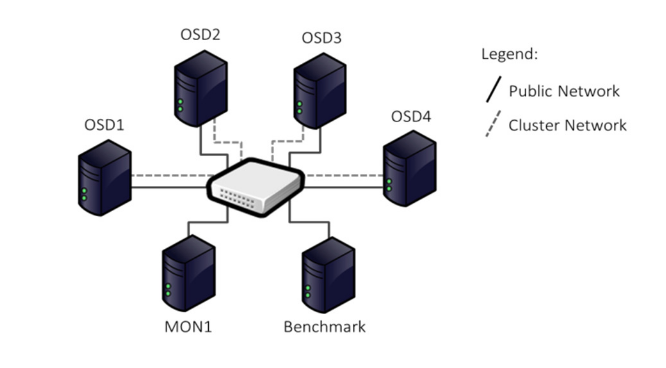
\includegraphics[scale=0.5]{doc/assets/images/Capitulo2/Esquema_conexion_EA.png}
    \caption{Esquema de interconexión que utiliza la prueba. Los OSD se interconcextan a dos redes /24 y estan separadas en VLANs \cite{7881982}.}
\end{figure}

\begin{figure}[H]
    \centering
    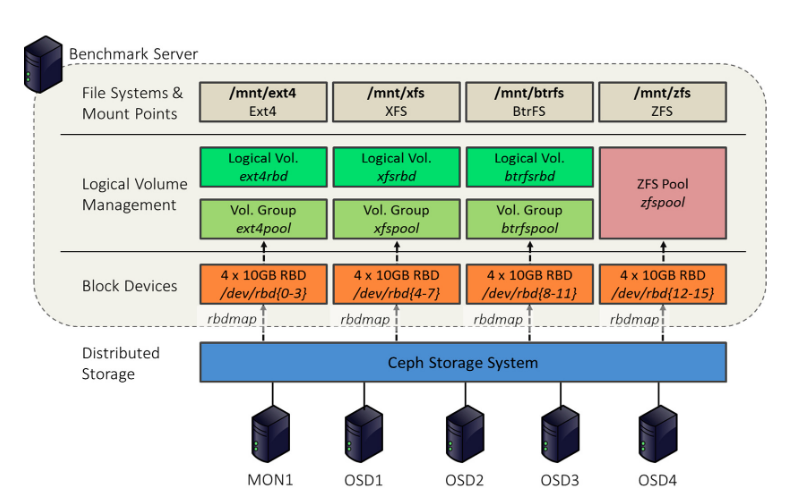
\includegraphics[scale=0.6]{doc/assets/images/Capitulo2/esquema_EA.png}
    \caption{Describe el servidor de benchmark con Ext4, XFS, BtrFS y ZFS que se ejecutan en  LVM y ZFS, con dispositivos de bloque RADOS (RBD) como dispositivos de bloque subyacentes en sustitución de discos físicos \cite{7881982}.}
\end{figure}

Referido al apartado de \textit{hardware setup} se encuentra muy completo, a falta de especificar el modelo y alguna característica reseñable de algún componente.

\subsubsection{Modern Filesystem Performance in Local Multi-disk Storage Space Configuration} 
Este documento incluye el análisis del rendimiento de S.A modernos en una configuración de almacenamiento multidisco.  En las pruebas se utilizan BTRFS, EXT4, XFS.  Las operaciones sobre los archivos se realizaron en varias configuraciones de almacenamiento utilizando Logical Volume Manager, que se diferenciaban por la política de asignación y la unidad de asignación de bloques.  En las configuraciones de almacenamiento se utilizan varios niveles de RAID. En el documento se expone la metodología de forma clara, y se tomará como referencia en este trabajo \cite{Smolinski2014ModernFP}.


\subsubsection{Conclusiones}
No sólo es importante definir que parámetros se van a considerar, o como se van a analizar, si no que también es vital concretar sobre qué hardware se ejecutan las pruebas. Desgraciadamente es bastante usual encontrar especificaciones incompletas, cómo pueden ser no especificar la frecuencia de refresco de la memoria RAM. Concretamente, esto ocurre en todos los trabajos citados anteriormente. Otro de los errores más comunes reside en ejecutar las pruebas en entornos virtualizados, es un error depender, en mayor o menor medida, del sistema hipervisor. Por último mencionar que la falta de definición de las cargas que ejecutan los benchmarks, imposibilita prácticamente por completo el análisis de resultados.\\

Después de analizar estas publicaciones y detectar algunos errores, se pondrá especial atención en ello para no repetirlos y los aspectos positivos se tomarán como referencia para realizar un trabajo de calidad.

%\textcolor{blue}{EL ESTADO DEL ARTE ES ENANO. HAY QUE AMPLIARLO ANALIZANDO FORTALEZAS Y DEBILIDADES DE CADA PAPER Y LUEGO HACIENDO UN PARRAFO FINAL RESUMEN COMO EL QUE YA HAS HECHO. TEN EN CUENTA QUE BASAS TU INVESTIGACION PARTIENDO DE LO QUE OTROS HAN HECHO, PARA ESO TIENES QUE EXPONER LAS CARACTERISTICAS DE LOS DEMÁS Y SACAR A RELUCIR EN LO QUE GANAS Y SI PIERDES EN ALGO. SE 100\% HONESTO :D}
